\subsubsection{Bivariate ridge trace plots}\label{sec:ridge2}

Ridge regression is touted (optimistically we think) as a method to counter the effects
of collinearity by trading off a small amount of bias for an
advantageous decrease in variance.  The results are often
visualized in a a \emph{ridge trace plot}
\citep{HoerlKennard:1970b},
showing the changes
in individual coefficient estimates as a function of $k$.
A bivariate version of this plot, with confidence ellipses for
the parameters is introduced here.  This plot provides greater
insight into the effects of $k$ on coefficient variance.\footnote{Bias and mean-squared error are a different matter: Although \citet{HoerlKennard:1970a} demonstrate that there is a range of values for the ridge constant $k$ for which the MSE of the ridge estimator is smaller than that of the OLS estimator, to know where this range is located requires knowledge of $\vec{\beta}$. As we explain in the following subsection, the constraint on $\vec{\hat{\beta}}$ incorporated in the ridge estimator can be construed as a Bayesian prior; the fly in the ointment of ridge regression, however, is that there is no reason to suppose that the ridge-regression prior is in general reasonable.}

Confidence ellipsoids for the OLS estimator are generated
from the estimated covariance matrix of the coefficients,
\begin{equation*}
\widehat{\Var} (\vec{\beta}^{\mathrm{OLS}}) = \hat{\sigma}^2_e (\mat{X}\trans \mat{X})^{-1} \period
\end{equation*}
For the ridge estimator, this becomes
%(Marquandt, 1970)
\citep{Marquardt:1970}
\begin{equation}
\widehat{\Var} (\vec{\beta}^{\mathrm{RR}}) = \hat{\sigma}^2_e
    [\mat{X}\trans \mat{X} + k \mat{I}]^{-1}
    (\mat{X}\trans \mat{X})
    [\mat{X}\trans \mat{X} + k \mat{I}]^{-1} \comma
%    = \mat{G}  (\mat{X}\trans \mat{X}) \mat{G} \comma
\end{equation}
which coincides with the OLS result when $k=0$.
	
\begin{figure}[htb!]
  \centering
  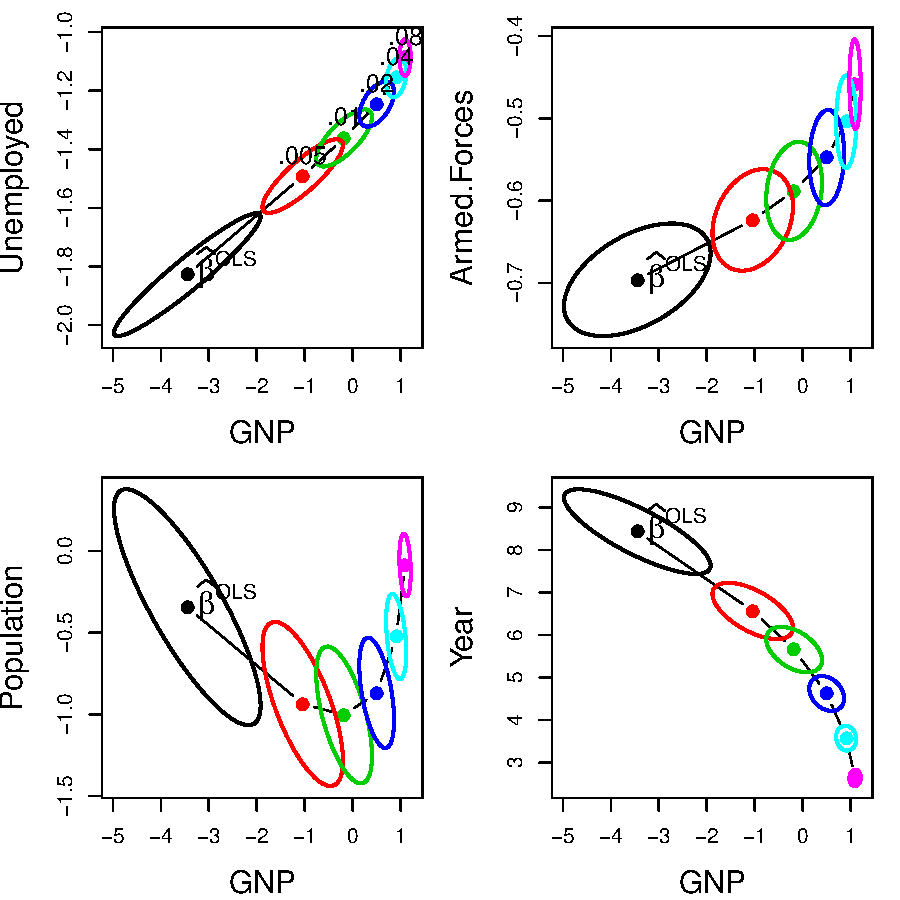
\includegraphics[width=\textwidth,clip]{fig/ridge2}
  \caption{Bivariate ridge trace plots for the coefficients of four predictors
  	against the coefficient for GNP in Longley's data, with
  	$k = 0, 0.005, 0.01, 0.02, 0.04, 0.08$.
  	In most cases the coefficients are driven toward zero, but the bivariate
  	plot also makes clear the reduction in variance.
  	To reduce overlap, all confidence ellipses are shown with 1/2 the standard radius.}%
  \label{fig:ridge2}
\end{figure}

\figref{fig:ridge2} uses the classic \citet{Longley:1967}
data to illustrate
bivariate ridge trace plots.  The data consist of an economic time series ($n=16$)
observed yearly from 1947 to 1962, with the number of people Employed as the
response and the following predictors:
GNP, Unemployed,  Armed.Forces,  Population,  Year, and GNP.deflator (using
1954 as 100).%
\footnote{
\citet{Longley:1967} used these data to demonstrate the effects of
numerical instability and round-off error in least squares computations
based on direct computation of the crossproducts matrix, $\mat{X}\trans\mat{X}$.
Longley's paper sparked the development of a wide variety of
numerically stable least squares algorithms (QR, modified Gram-Schmidt, etc.)
now used is almost all statistical software.
Even ignoring numerical problems
(not to mention problems due to lack of independence), these
data would be anticipated to exhibit high collinearity because
a number of the predictors would be expected to have strong associations
with year and/or population, yet both of these are also included among the
predictors.
}
The standard linear model for these data, in R notation,
is \verb|lm(Employed ~ ., data=longley)|, where ``\texttt{.}''  in the model formula means
``all other variables'' in the data set as predictors.  
For each value of $k$, the plot
shows the estimate $\widehat{\vec{\beta}}$, together with the confidence
ellipse.  For the sake of this example, we assume that GNP is a primary
predictor of Employment, and we wish to know how other predictors modify the
regression estimates and their variance when ridge regression is used.

For these data, it can be seen that even small values of $k$ have substantial
impact on the estimates $\widehat{\vec{\beta}}$. What is perhaps more dramatic
(and unseen in univariate trace plots) is the impact on the size of the confidence
ellipse.  Moreover, shrinkage in variance is generally in a similar direction to the
shrinkage in the coefficients.
